\chapter{Roboterbewegung im Occupancy Grid}
Die physikalische Umgebung des Roboters wird diskretisiert durch das \textit{Occupancy Grid}, ein binärer, zweidimensionale Raum aus der Vogelperspektive. Implementiert mit der Python Bibliothek \textit{Numpy}, hat das Boolean Array \texttt{occupancy\_grid[Y][X]} die Länge \texttt{occupancy\_grid\_length} und Breite \texttt{occupancy\_grid\_width} und den Ursprung links oben. Jede Koordinate ist entweder durch ein Hindernis belegt (\texttt{occupancy\_grid[Y][X] == False}) oder frei von Hindernissen (\texttt{occupancy\_grid[Y][X] == True}).

Im Occupancy Grid gibt es drei Roboterpositionen: \texttt{start\_point}, \texttt{current\_position} und \texttt{goal\_point}.
\begin{figure}[H]
	\small
	\centering	
	\hspace*{\fill}
	\begin{minipage}{0.5\textwidth}%
		\begin{minted}[
			obeytabs=true,
			tabsize=2,
			autogobble,
			fontsize={\fontsize{6.8}{7.1}\selectfont},
			frame=single
			]{python}
			occupancy_grid = 
			[[T, T, T, T, T, T, T, T, T, T, T, T, T, T, T, T, T, T, T, T],
			 [T, T, T, T, T, T, T, T, T, T, T, T, T, T, T, T, T, T, T, T],
			 [T, T, T, T, T, T, T, T, T, T, T, T, T, T, T, T, T, T, T, T],
			 [T, T, T, T, T, T, T, T, T, T, T, T, T, T, T, T, T, T, T, T],
			 [T, T, T, T, T, T, T, T, T, T, T, T, T, T, T, T, T, T, T, T],
			 [T, T, T, T, T, T, T, T, T, T, T, T, T, T, T, T, T, T, T, T],
			 [T, T, T, T, T, T, T, T, T, T, T, T, T, T, T, T, T, T, T, T],
			 [T, T, T, T, T, T, T, T, T, T, T, T, T, T, T, T, T, T, T, T],
			 [T, T, T, T, T, T, T, T, T, F, F, T, T, T, T, T, T, T, T, T],
			 [T, T, T, T, T, T, T, T, T, F, F, T, T, T, T, T, T, T, T, T],
			 [T, T, T, T, T, T, T, T, T, T, T, T, T, T, T, T, T, T, T, T],
			 [T, T, T, T, T, T, T, T, T, T, T, T, T, T, T, T, T, T, T, T],
			 [T, T, T, T, T, T, T, T, T, T, T, T, T, T, T, T, T, T, T, T],
			 [T, T, T, T, T, T, T, T, T, T, T, T, T, T, T, T, T, T, T, T],
			 [T, T, T, T, T, T, T, T, T, T, T, T, T, T, T, T, T, T, T, T],
			 [T, T, T, T, T, T, T, T, T, T, T, T, T, T, T, T, T, T, T, T],
			 [T, T, T, T, T, T, T, T, T, T, T, T, T, T, T, T, T, T, T, T],
			 [T, T, T, T, T, T, T, T, T, T, T, T, T, T, T, T, T, T, T, T],
			 [T, T, T, T, T, T, T, T, T, T, T, T, T, T, T, T, T, T, T, T]]
		\end{minted}
	\end{minipage}
	\hspace*{\fill}
	\begin{minipage}{0.35\textwidth}%
		\footnotesize
		\resizebox{\linewidth}{!}{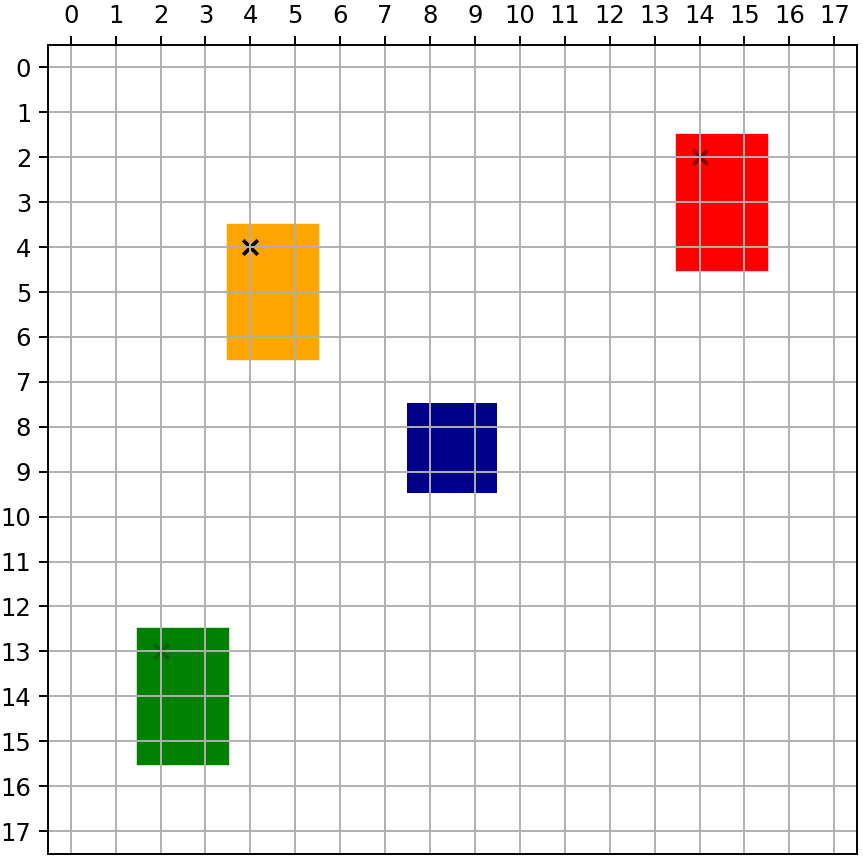
\includegraphics{bilder/occupancy-grid3.png}}
	\end{minipage}
	\hspace*{\fill}
	%	\vspace{-1cm}
	\caption{Ein einfaches Occupancy Grid mit vier Hindernissen, dem \texttt{start\_point} bei (\texttt{X=2}, \texttt{Y=13}), der \texttt{current\_position} bei (\texttt{X=4}, \texttt{Y=4}) und dem \texttt{goal\_point} bei (\texttt{X=14}, \texttt{Y=2})}.
\end{figure}

\vspace*{-0.3cm}
Die Dimension des Roboters wird durch die Variablen \texttt{robot\_width} und \texttt{robot\_length} definiert. Pro Verarbeitungseinheit kann sich der Roboter relativ zum \textit{Ankerpunkt} der aktuellen Position entweder durch eine Translation oder Rotation im Occupancy Grid bewegen:
\begin{itemize}
\item \textbf{Translation} nach links (\texttt{x-1}), rechts (\texttt{x+1}), oben (\texttt{y-1}) und unten (\texttt{y+1})
\item \textbf{Rotation} um den Ankerpunkt. Bei einer Rotation von $0$° liegt dieser Referenzpunkt in der linken oberen Koordinate innerhalb der Roboterdimensionen.
\end{itemize}
\vspace*{0.3cm}
\begin{figure}[H]
	\centering
	\footnotesize
	\centerline{\resizebox{1\linewidth}{!}{\input{bilder/robotermodell_latex.pdf_tex}}}
	\caption{Bewegung eines Roboters mit variabler Dimension durch Translation und Rotation.}
\end{figure}

